\addcontentsline{toc}{chapter}{Занятие 12. Проверка параметрических гипотез.
                              Критерий Неймана-Пирсона}
\chapter*{Занятие 12. Проверка параметрических гипотез. Критерий Неймана-Пирсона}

\addcontentsline{toc}{section}{Контрольные вопросы и задания}
\section*{Контрольные вопросы и задания}

\subsubsection*{Что называется статистической гипотезой?}

Статистическая гипотеза --- предположение о виде распределения и свойствах случайной величины,
которое можно подтвердить или опровергнуть применением статистических методов к данным выборки.

\subsubsection*{Какую гипотезу называют основной, альтернативной, простой, сложной?}

Нулевая гипотеза --- гипотеза, подлежащая проверке.
Альтернативная гипотеза --- каждая допустимая гипотеза, отличная от нулевой.
Нулевую гипотезу обозначают $H_0$, альтернативную ---
$H_1$ (от Hypothesis --- <<гипотеза>> (англ.)).

Простой гипотезой называют предположение, состоящее в том,
что неизвестная функция $F \left( t \right) $
отвечает некоторому совершенно конкретному вероятностному распределению.

Сложной гипотезой называют предположение о том,
что неизвестная функция $F \left( t \right) $ принадлежит некоторому множеству распределений,
состоящему из более чем одного элемента.

\subsubsection*{Что такое статистический критерий?}

Статистический критерий --- строгое математическое правило,
по которому принимается или отвергается та или иная статистическая
гипотеза с известным уровнем значимости.

\subsubsection*{Что такое уровень занчимости критерия для проверки статистической гипотезы?}

Можно отвергнуть гипотезу $F_1$, когда она будет верна.
В случае простой гипотезы $F_1$ вероятность ошибки равна  $P_{F_1} \left( \vec{X} \in D \right) $.
Эту вероятность называют уровнем значимости статистического критерия.

\subsubsection*{Какое множество называют критическим для проверки статистической гипотезы?}

Критическая область --- это совокупность значений статистики, которые <<говорят>>,
что нулевую гипотезу следует отвергнуть.

\subsubsection*{В чём состоит ошибка первого рода, второго рода?}

$1 - \alpha = P \left( H_1 \; \middle| \; H_0 \right) $ --- ошибка первого рода.
Означает, что отклонили нулевую гипотезу в то время, как на самом деле она истинна.

$ \beta = P \left( H_0 \; \middle| \; H_1 \right) $ --- ошибка второго рода.
Это означает принять нулевую гипотезу, которая на самом деле ложна.

\subsubsection*{Что называют мощностью критерия?}

$1 - \beta $ --- мощность критерия.

\subsubsection*{Сформулируйте критерий согласованности Колмогорова,
                критерий согласованности $ \chi^2$ Пирсона, лемму Неймана-Пирсона}

\textit{Критерий Колмогорова-Смирнова.}
Если $F$ --- непрерывное распределение,
то
$ \sqrt{n} \cdot
  \sup \limits_{ \mathbb{R}} \left[ F_n \left( x \right) - F \left( x \right) \right] \approx
  D_{ \theta }$
--- известное распределение.

\textit{Критерий Пирсона (критерий согласия $ \chi^2$).} Есть выборка $X_1, \dotsc, X_n$.
Имеет ли оа распределение $F$?
Попробуем устроить дискретную процедуру.
Разбиваем интервал возможных значений выборки на $N$ полуинтервалов (чисел, частей) ---
рис. \ref{fig:12}.

\begin{figure}[h!]
  \centering
  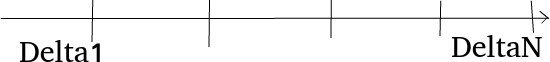
\includegraphics[width=.4\textwidth]{./pictures/12.png}
  \caption{Возможные значения выборки}
  \label{fig:12}
\end{figure}

Обозначим через $p_i = P_F \left( X_1 \in \Delta_i \right) > 0$.

Количество элементов выборки, которые попали в $ \Delta_i$, обозначим через
$$ \nu_i =
  \sum \limits_{k = 1}^n \mathbbm{1}_{ \Delta_i} \left( X_k \right).$$
Рассмотрим сумму
$$ \sum \limits_{i = 1}^n \frac{ \left( \nu_i - np_i \right)^2}{np_i} \approx
  \chi_{n - 1}^2$$
при $n \to \infty $ (после применения центральной предельной теоремы).

Все $ \nu_i$ в сумме дают $n$, следовательно, есть связь,
то есть $ \left( n - 1 \right) $-на степень свободы.

Так происходит, если угадали $p_i$, иначе --- выражение быстро растёт.

\textit{Лемма Неймана-Пирсона.}
$D_{C_{ \alpha }}$ --- оптимально, то есть для произвольной $D$,
такой что $P_{F_1} \left( D^C \right) = \alpha $, оказывается,
что $P_{F_2} \left( D \right) = P_{F_2} \left( D_{C_{ \alpha }} \right) $, то есть утверждается,
что множество уровня является оптимальным.

\addcontentsline{toc}{section}{Аудиторные задачи}
\section*{Аудиторные задачи}

\subsubsection*{12.3}

\textit{Задание.}
Пусть $X_1, \dotsc, X_{100}$ ---
независимые наблюдения нормального распределения с параметрами $ \left(m, 4 \right) $.
Постройте критерий Неймана-Пирсона с уровнем доверия $ \alpha = 0.95$ для проверки гипотезы
$ \left\{ H_0: \, m = 0 \right\} $ против альтернативы $ \left\{ H_1: \, m = 1 \right\} $.
Вычислите мощности этого критерия.

\textit{Решение.} $X_1, \dotsc, X_{100} \sim N \left( m, 4 \right) $.

Нулевая гипотеза $H_0$ --- это $m = 0$ против альтернативы $H_1: \, m = 1$.

Вычисляем функцию правдоподобия
$$L \left( \vec{X}, m \right) =
  \prod \limits_{i = 1}^{100}
    \frac{1}{ \sqrt{2 \pi } \cdot 2} \cdot e^{- \frac{ \left( X_i - m \right)^2}{2 \cdot 4}} =
  \left( \frac{1}{2^{ \frac{3}{2}} \sqrt{ \pi }} \right)^{100} \cdot
  e^{- \frac{ \sum \limits_{i = 1}^{100} \left( X_i - m \right)^2}{8}}.$$

Отношение правдоподобий
$$ \varphi \left( \vec{X} \right) =
  \frac{e^{- \frac{ \sum \limits_{i = 1}^{100} \left( X_i - 1 \right)^2}{8}}}{e^{- \frac{ \sum \limits_{i = 1}^{100} X_i^2}{8}}} =
  e^{- \frac{1}{8} \left[ \sum \limits_{i = 1}^{100} \left( X_i - 1 \right)^2 + \sum \limits_{i = 1}^{100} X_i^2 \right] } =
  e^{ \frac{ \sum \limits_{i = 1}^{100} X_i}{4} - \frac{100}{8}} =
  e^{25 \overline{X} - 12.5}.$$

Сумма $X_i$ должна превысить какой-то уровень,
тогда $ \varphi \left( \vec{X} \right) $ будет превышать какой-то уровень.

$ \left\{ \overline{X} > c \right\} $ --- критическая область для $H_0$, где $c$ находим из условия,
что $P \left( \overline{X} > c \; \middle| \; H_0 \right) = 0.05$.

При гипотезе $H_0, \, X_i$ имеет распределение $N \left( 0, 4 \right) $.
Тогда $ \xi = \overline{X}$ будет иметь распределение
$$N \left( 0, \frac{4}{100} \right) =
  N \left( 0, \frac{1}{25} \right),$$
а значит $5 \overline{X} \sim N \left( 0, 1 \right) $ --- стандартный нормальный закон.
Теперь можем вычислить $c$.

Вычисляем вероятносить
$P \left( \xi > c \right) =
  P \left( 5 \xi > 5c \right) =
  0.05 =
  \Phi_t \left( 5c \right) $.
Отсюда из таблицы $5c = 1.65$, откуда $c = 0.33$.
Таким образом, если $ \overline{X} < 0.33$, то отклоняем основную гипотезу,
принимаем альтернативную, то есть говорим, что $m = 1$.

Если же $ \overline{X} \leq 0.33$, то нет причин отклонять основную гипотезу,
то есть принимаем $m = 0$.

Итак, сформулировали критеий.

Вычисляем
$ \beta =
  P \left( H_0 \; \middle| \; H_1 \right) =
  P \left( \overline{X} < 0.33 \; \middle| \; H_1 \right) $.
При $H_1 \, X_i \sim N \left( 1, 4 \right) $.
Тогда
$$ \overline{X} \sim
  N \left( 1, \frac{1}{25} \right).$$
Значит, $5 \left( \overline{X} - 1 \right) \sim N \left( 0, 1 \right) $.
Получаем
$$P \left( \overline{X} < 0.33 \; \middle| \; H_1 \right) =
  P \left( 5 \left( \overline{X} - 1 \right) < -0.67 \cdot 5 \right) =
  P \left( 5 \left( \overline{X} - 1 \right) < -3.35 \right).$$
Пользуемся таблицей нормального распределения
$$P \left( 5 \left( \overline{X} - 1 \right) < -3.35 \right) =
  \Phi_t \left( 3.35 \right) <
  \Phi_t \left( 3 \right) =
  0.00135.$$

А значит, мощность $1 - \beta > 1 - 0.00135$ --- очень близкое число к единице, что хорошо.

\addcontentsline{toc}{section}{Домашнее задание}
\section*{Домашнее задание}
